\chapter{Second-order FV with Malpasset}

\section{Introduction}

Free-surface shallow-flow models can be applied across a wide range of scenarios to simulate flood events, tsunami, and the consequences of dam collapse. Amongst the most advanced models are Godunov-type schemes, allowing accurate simulation even where complex flow dynamics exist (e.g. hydraulic jumps), and utilising high-resolution datasets available at low expense with LiDAR data. Auspicious engineering design and risk analysis increasingly demands these high levels of detail and accuracy \citep{French2003,Haile2005,Marks2000}. To capture highly transient complex hydrodynamic processes, e.g. those induced by dam breaks, a Godunov-type scheme is normally developed using an explicit scheme in time integration, which imposes a strict constraint on the timestep. However, these explicit time-marching schemes are computationally expensive, thus high-resolution simulations across large catchment or city scales are often unfeasible in practice without super-computers, despite recent substantial developments in CPU power. This deficiency is especially pertinent for natural flood management techniques, whereby small runoff storage and attenuation features are distributed throughout a catchment, as shown to be effective in pilot projects in small catchments such as Belford, Northumberland \citep{EnvironmentAgency2012,Wilkinson2010}. Computational models do not yet exist with sufficient physical basis to scientifically elucidate the practice and establish how to upscale the approach to much larger catchments. New approaches are required which can expedite simulations without compromising the numerical representation of the underlying physical processes, if we are to provide the necessary scientific basis, understanding, and guidance for applying this cost-effective approach elsewhere. 

To overcome computational constraints, numerous types of acceleration have been explored previously. Simplification of the numerical representation often provides inaccurate velocities, therefore compromising the temporal accuracy of the solution \citep{Pender2010,Singh1996,Neelz2009}, and may neglect important phenomena such as backwater effects; dynamic grid adaptation delivers limited benefits (2-3x faster) for complex flow characteristics and introduces challenges for managing mass and momentum conservation during refinement \citep{Liang2004}; many high-performance computing (HPC) techniques such as distributed computing (e.g. Condor) are constrained by communication because of the interdependency of the solution between cells and their neighbours, making scalable implementations difficult to accomplish \citep{Pau2006,Delis2009}. 

-- SNIP --

GPUs provide an excellent ratio of computing power to cost, making them a potential future tool for engineering consultancies, but commercially viable software must be resilient to hardware differences in capacities and architectures. An appropriate scheme for application across a wide range of scenarios must also be able to preserve depth positivity, capture shocks (flow discontinuities), appropriately manage wet-dry interfaces, and handle complex domain topography or exhibit the so-called well-balanced property \citep{Xing2010,Murillo2010}. 

Few generalised modelling tools with all these qualities currently exist. Herein we develop software that does boast all of the aforementioned qualities to provide a next-generation shallow-flow modelling tool that can readily be applied for different purposes (i.e. different flood simulations and catchment modelling) and can easily be optimised for a wide range of different GPUs and CPUs without compromising on accuracy, functionality or the robustness of the solution. Through application to a real-world dam-break event, one of the most difficult types of flood scenario to accurately simulate, we demonstrate that high levels of performance are achievable even with a complex Godunov-type scheme and an HLLC Riemann solver. 

\section{Review of a finite-volume Godunov-type scheme}

The conservative form of the shallow water equations (SWEs) can be obtained by depth-integration of the Reynolds-averaged Navier-Stokes equation, to give a hyperbolic conservation law defined as
\begin{equation}
	\label{SWE}
	\frac{\partial\textbf{U}}{\partial t} +
	\frac{\partial\textbf{F}}{\partial x} +
	\frac{\partial\textbf{G}}{\partial y} =
	\textbf{S} ,
\end{equation}
where \(\textbf{U}\) is a vector of conserved variables, \(\textbf{F}\) and \(\textbf{G}\) are vectors of fluxes in \(x\)- and \(y\)-directions, and \(\textbf{S}\) is a vector of source terms. The values of \(t\), \(x\), and \(y\) represent time and the two Cartesian coordinates respectively. Herein we neglect the viscous fluxes, surface stresses and Coriolis effects to give vectors
\renewcommand{\arraystretch}{1.5}
\begin{equation}
	\label{SWETerms}
	\begin{alignedat}{2}
		&\textbf U && = \left[ \begin{array}{c}
			\eta \\
			uh \\
			vh
		\end{array} \right] ,\\
		&\textbf F &&  = \left[ \begin{array}{c}
			hu \\
			hu^2 + \frac{1}{2}(g\eta^2 - 2\eta z_b) \\
			huv
		\end{array} \right] ,\\
		&\textbf G && = \left[ \begin{array}{c}
			hv \\
			hvu \\
			hv^2 + \frac{1}{2}(g\eta^2 - 2\eta z_b) \\
		\end{array} \right] ,\\
		&\textbf S && = \left[ \begin{array}{c}
			0 \\
			-\frac{\tau_bx}{\rho} - g\eta \frac{\partial z_b}{\partial x} \\
			-\frac{\tau_by}{\rho} - g\eta \frac{\partial z_b}{\partial y} \\
		\end{array} \right] .
	\end{alignedat}
\end{equation}
Here, \(\eta\) is the free-surface level above datum; \(u\) and \(v\) are depth-averaged velocities in the \(x\)- and \(y\)-directions respectively; \(h\) is the water depth; \(uh (=q_x)\) and \(vh (=q_y)\) are unit-width discharges; \(g\) is the acceleration due to gravity; \(\rho\) is the water density; \(\tau_{bx}\) and \(\tau_{by}\) are bed stresses in the two directions; and \(z_b\) is the bed elevation above datum. The deviatory vector forms displayed here ensure the equations exhibit the well-balanced property and thereby provide the correct behaviour for a lake-at-rest case with uneven bed topography \citep{Liang2009c}.

\subsection{Finite-volume Godunov-type scheme}

A Godunov-type scheme \citep{Godunov1959} is used to solve \eqref{SWE} by computing fluxes through local Riemann solutions at each cell interface. Flux differences along each axis are then used to update flow variables in each cell with the time-marching formula, 
\begin{equation}
	\label{GodunovUpdate}
	\begin{alignedat}{2}
	\textbf{U}^{t+\Delta t} = \textbf{U}^t & - \frac{\Delta t}{\Delta x}(\textbf{F}^+ - \textbf{F}^-) \\
					     &  - \frac{\Delta t}{\Delta y}(\textbf{G}^+ - \textbf{G}^-) + \Delta t \textbf{S} , 
	\end{alignedat}
\end{equation}
where \(\textbf{F}^-\), \(\textbf{F}^+\), \(\textbf{G}^-\), \(\textbf{G}^+\)  are fluxes through a cell's western, eastern, southern and northern interfaces respectively; and \(\Delta x\) and \(\Delta y\) are cell dimensions in each respective direction. The HLLC (i.e. Harten, Lax, van Leer, contact-restoration) solver \citep{Toro1994} is used for approximate Riemann solutions, with less computational burden than an exact solution but an appropriate degree of accuracy for most shallow flow simulations \citep{Erduran2002,Zoppou2003}.

Snipped.

\subsection{Depth positivity preservation}

Non-negative reconstruction is required before computing Riemann solutions to ensure depth positivity is preserved. The approach adopted herein is appropriate for flood modelling \citep{Liang2010a}. In the context of a finite-volume Godunov-type scheme, after linear reconstruction of flow variables and the bed elevation for the cell interface under consideration, an intermediary bed elevation is obtained, where \(\tilde{ }\) denotes a variable before non-negative reconstruction and subscript \(L\) or \(R\) denote sides of the interface,
\begin{equation}
	\label{NonNegRec1}
	\hat{z}_b = max(\tilde{z}_{b,L}, \tilde{z}_{b,R}) ,
\end{equation}
from which the final reconstructed variables can be computed at both sides of the interface. Velocities are unchanged and used to compute new unit-width discharge with the reconstructed depth and free-surface level,
\begin{equation}
	\label{NonNegRec2}
	\begin{alignedat}{2}
		&h && = max(0, \tilde{\eta} - \hat{z}_b) ,\\
		&\hat{\eta} && = h + \hat{z}_b .
	\end{alignedat}
\end{equation}
Finally, a local bed modification is applied to datum-dependent variables to ensure the free-surface level is not below the bed elevation \citep{Liang2010},
\begin{equation}
	\label{NonNegRec3}
	\begin{alignedat}{2}
		&\Delta z && = max(0, \hat{z}_b - \tilde{\eta}_L) ,\\
		&z_b      && = \hat{z}_b - \Delta z               ,\\
		&\eta     && = \hat{\eta} - \Delta z              .
	\end{alignedat}
\end{equation}
The reconstructed flow variables resulting from \eqref{NonNegRec2} and \eqref{NonNegRec3} together with the unit-width discharges become the states defining the local Riemann problem across the cell interface, which is subsequently solved using an HLLC approximate Riemann solver to give the interface fluxes for updating the flow variables to a new time step using \eqref{GodunovUpdate}.

\subsection{Stability criterion}

Snipped. The Courant number is set to 0.5 for simulations herein. 

\subsection{Implicit friction solution}

Snipped.

\section{GPU-based implementation}

Snipped.

\subsection{Memory management}

Snipped.

Snipped.

\subsection{Timestep reduction}

A single timestep is used for all cells, identified from the smallest permissible timestep in the domain. A kernel that iterates through every cell serially is highly inefficient (Amdahl's Law), hence a two-stage reduction is used here to capitalise on the parallel nature and power of the processing units. A fixed global work size is selected and used as the stride through the global array of cell data, with each work-item identifying the smallest timestep from those cells it examines. Each work-item commits this data to an array in local memory and binary comparison is carried out within each work-group, starting at the middle, progressing towards the first element, with work-items successively retired. The first work-item in a work-group commits the lowest timestep identified in the group to a much smaller global array, which is examined by the single instance of the kernel for advancing the overall simulation time. This process is represented in Fig. \ref{ReductionProcess}. The global work size provides a method of controlling the workload assigned to each work-item.

\begin{figure*}[tpb]
\centering
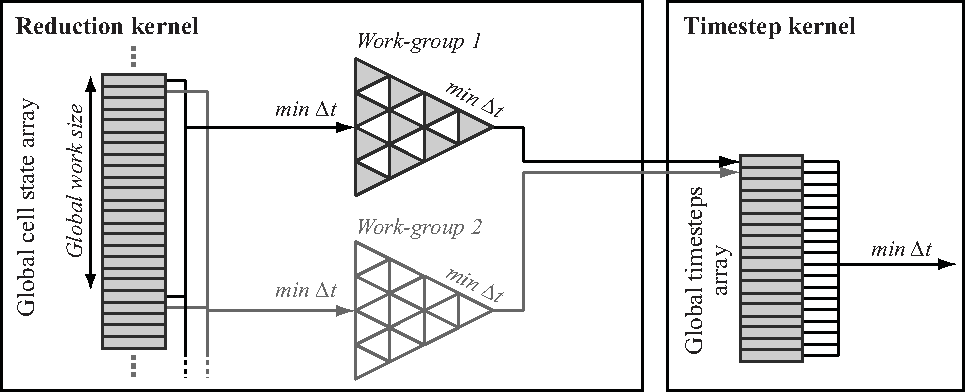
\includegraphics[width=1.0\textwidth]{heterogeneous-dev-figures/Figure_6_Greyscale.pdf}
\caption{Simplified representation of the two-stage timestep reduction process, with only the first two work-groups indicated.}
\label{ReductionProcess}
\end{figure*}

\subsection{Kernel scheduling and reduction control}

Snipped.

\begin{figure*}[tpb]
\centering
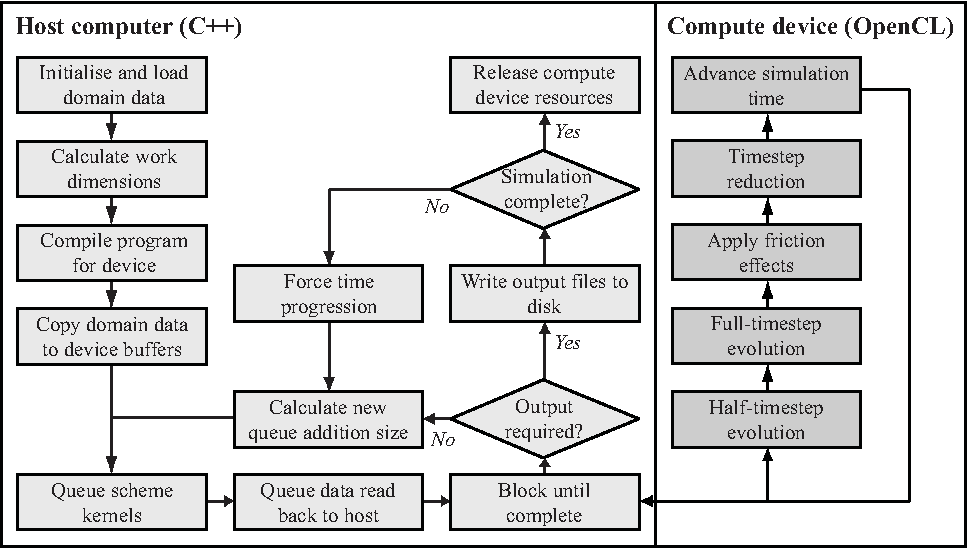
\includegraphics[width=1.0\textwidth]{heterogeneous-dev-figures/Figure_7_Greyscale.pdf}
\caption{Flowchart of main operations on the host computer and compute device.}
\label{ComputerDeviceInteraction}
\end{figure*}

\section{Results and discussion}

Snipped.

\section{Conclusions}

In this paper, we have presented how the shallow water equations can be efficiently solved with second-order accuracy using a finite-volume Godunov-type scheme and GPUs. Factors affecting GPU performance are considered and a range of corresponding configuration parameters devised to allow the software to be used and optimised with a wide range of modern processors. Simulations of a real-world dam collapse event with the new framework were shown to exhibit good agreement with a post-event survey, without compromising accuracy but still providing significant performance improvements against a CPU. The results demonstrate that the software developed herein is appropriate for simulating some of the most challenging flood events, where shock-like flow discontinuities are present. The new approach will facilitate simulations at resolutions previously unfeasible across whole cities and large catchments. As further work, we propose to extend the software to take advantage of multiple GPUs in a single host computer to facilitate further performance improvements and greater numbers of cells.

32-bit floating-point simulations are shown to introduce significant but localised errors to results; 64-bit is therefore recommended for flood modelling. Caching cell data to local memory provided no direct performance benefit for any of the devices used. Where local memory is used, reducing bank conflicts with array padding is shown to reduce simulation times slightly.
